\documentclass{report}
\usepackage{graphicx}
\graphicspath{ {./images/} }
\usepackage[nottoc]{tocbibind}
\usepackage{blindtext}
\usepackage{booktabs}% http://ctan.org/pkg/booktabs
\newcommand{\tabitem}{~~\llap{\textbullet}~~}
\usepackage{geometry}
\geometry{
	a4paper,
	total={170mm,257mm},
	left=30mm,
	right=30mm,
	top=20mm,
}
\usepackage{array}
\usepackage{listings}
\usepackage{xcolor}
\definecolor{mygray}{rgb}{0.9,0.9,0.9}
\lstset{
	tabsize=3,
	basicstyle={\small\ttfamily},
	backgroundcolor=\color{mygray}
}

\begin{document}
	\begin{titlepage}
		\centering
		
\includegraphics[width=0.5\textwidth]{unipi.png}\par\vspace{1cm}
		{\scshape\LARGE Department of Information Engineering \par}
		\vspace{1cm}
		{\huge\bfseries Information Systems \par Task 1 Documentation  \par}
		\vspace{2cm}
		\vfill
		{\Large\scshape Students: \par 
			Adriano Botti \par
			Antonio Le Caldare \par
			Francesco Merola \par 
			Giacomo Ponziani \par}
		\vfill
		
	\end{titlepage}
\tableofcontents
\newpage
\listoffigures

\addcontentsline{toc}{chapter}{Application Specifications}
\chapter*{Application Specifications}
The goal of the application that we implemented is to provide a way for both students and professors to manage the registration process for exams. More specifically, we want the application to exert the following functionalities:
\begin{itemize}
	\item For Students:
	\begin{enumerate}
		\item Check past exams results
		\item Register to an exam date
		\item Delete an exam registration
	\end{enumerate}
	\item For Professors:
	\begin{enumerate}
		\item Add grades to an exam
		\item Create a new exam date
	\end{enumerate} 
\end{itemize}
%The application is realized using the Java language, with the JavaFX extension to manage a graphic interface. The back-end uses a MySQL database to store the information.

\addcontentsline{toc}{chapter}{Requirements and Use Cases}
\chapter*{Requirements and Use Cases}
\addcontentsline{toc}{section}{Functional Requirements}
\section*{Functional Requirements}
The Professor:
\begin{enumerate}
	\item shall be able to insert an exam, associated with a course he holds, in a date of choice
	\item shall not be able to inster an exam for a date precedent to the current date
	\item shall be able to insert the corresponding grade for a student in their registration for that exam.
	\item shall insert all grades in the exact date of the exam
\end{enumerate}
The Student:
\begin{enumerate}
	\item shall be able to check the results of past exams
	\item shall be able to register to an exam not yet took
	\item shall not be able to register to an exam after the exam date.
	\item shall be able to register to more successive exams for the same course
	\item If the student registered to successive exams for the same course he just got a mark for, then those future registrations shall be hidden
	\item shall be able to deregister from an exam he was previously registered to
	\item shall not be able to deregister from an exam alredy took
	\item shall not be able to deregister from an exam after the exam date.
\end{enumerate}
\addcontentsline{toc}{section}{Non-Functional Requirements}
\section*{Non-Functional Requirements}
For the application we identified Consistency and Availability as the two most important non-functional requirements.
%Both the requirements can be satisfied by the use of a RDBMS, since for our application we don't manage high volumes of data. For this reason we employed a MySQL DBMS to implement our back-end
\newpage
\addcontentsline{toc}{section}{Use Case Diagram}
\section*{Use Case Diagram}
\begin{figure}[ht]
	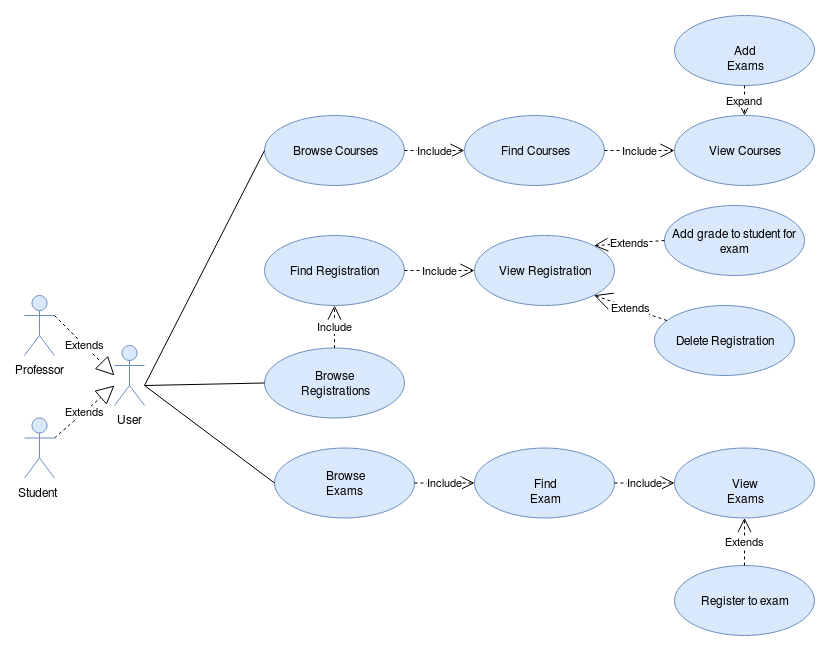
\includegraphics[width=0.9\textwidth]{UseCaseDiagram.png}
	\caption{Use Case Diagram}
\end{figure}

\begin{itemize}
	\item \textbf{Add Exam} : This operation can only be performed by a Professor.\\ He/She will be able to browse his/her tenured courses, select the one to add a new exam to and then add it.
	\item \textbf{Add Grade} : This operation can only be performed by a Professor.\\ He/She will be able to browse the registrations for his/her tenured courses, select the registration to add a grade to and then add it.
	\item \textbf{Register to Exam} : This operation can only be performed by a Student.\\ He/She will be able to browse all the exams to which is possible to register, select one and perform the registration.
	\item \textbf{Deregister to Exam} : This operation can only be performed by a Student.\\ He/She will be able to browse his/her active registrations, select one and deregister from it.
	\item \textbf{See Grades} : This operation can only be performed by a Student.\\ He/She will be able to browse his/her registrations and show only the one with a sufficient.
\end{itemize}
For more detail and a step-by-step description of the different scenarios, see chapter \textit{User's Manual}.
\newpage

\addcontentsline{toc}{chapter}{UML Class and Entity-Relationship Diagrams}
\chapter*{UML Class and Entity-Relationship Diagrams}
\addcontentsline{toc}{section}{UML Class Diagram}
\section*{UML Class Diagram} 
The UML Class Diagram shows the main objects involved in our application, with the respective logical relationships.
\begin{figure}[ht]
	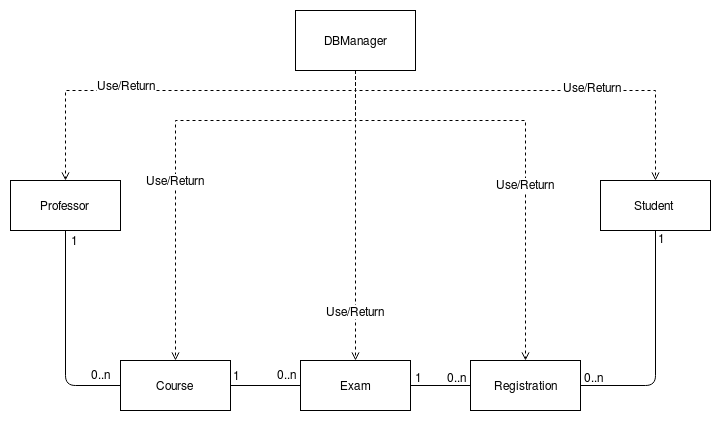
\includegraphics[width=0.6\textwidth]{ClassDiagram.png}
	\caption{UML Class Diagram}
\end{figure} 
From this model we derived an Entity-Relationship Diagram, where the dependecies are more deeply identified. Finally we will show the final database schema implemented on the MySQL RDBMS.
\addcontentsline{toc}{section}{ER Vocabulary}
\section*{ER Diagram}
\subsection*{Names definition}
Here we define in detail the terms for the main entites and relationships we will use in the following:
\begin{itemize}
	\item \textit{Student}\\ A student is an entity which is able to perform the operations already defined in the requirements. He's an actor for our application. 	
	\item \textit{Professor}\\ A professor is an entity which is able to perform the operations already defined in the requirements. He's an actor for our application. 	
	\item \textit{Course}\\ A course is held by one and only one professor. The course object only includes information about its name, cfu and the helding professor. It holds no information about when exams for that course will take place. 	
	\item \textit{Exam}\\ An exam represents the actual date of the examination for a course.
	\item \textit{Exam Result} An exam result relates an exam to all the students who registered to that exam, adding the information of the grade, if meaningful.\\
\end{itemize} 
\newpage
\subsection*{Entities}
\begin{table}[ht]
	\centering
	\begin{tabular}{| m{6em} | m{15em} | m{8em} |}
		\hline
		\textbf{Entity} & \textbf{Description} & \textbf{Attributes} \\
		\hline
		Student & Holds all the information related to the students & 
		\tabitem $\underline{id}$ \\
		 & &\tabitem $name$ \\
		 & &\tabitem $surname$ \\
		\hline
		Professor & Holds all the information related to the professors & 
		\tabitem $\underline{id}$ \\
		& &\tabitem $name$ \\
		& &\tabitem $surname$ \\
		\hline
		Course & Holds the information related to the courses & 
		\tabitem $\underline{id}$ \\
		& &\tabitem $name$ \\
		& &\tabitem $cfu$ \\
		& &\tabitem $professor$ \\
		\hline
		Exam & Holds all the new and past exams& 
		\tabitem $\underline{course (ext)}$ \\
		& &\tabitem $\underline{date}$ \\
		\hline
	\end{tabular}
\end{table}
\vspace{10em}
\subsection*{Relationships}
\begin{table}[h]
	\centering
	\begin{tabular}{| m{6em} | m{14em} | m{8em} | m{7em} |}
		\hline
		\textbf{Relationship} & \textbf{Description} & \textbf{Participants} & \textbf{Attributes} \\
		\hline
		Teaching & Links Professors to their held courses & 
		\tabitem Professor(1,N) & \\ & &
		\tabitem Course(1,1) & \\
		\hline
		Exam Result & Links students to exams, with the respective grade & 
		\tabitem Student(0,N) & \tabitem $grade$ \\ & &
		\tabitem Exam(0,N) & \\
		\hline
		Exam Date Creation & Links the courses to the exams through a date & 
		\tabitem Course(0,N) & \\ & & 
		\tabitem Exam(1,1) & \\
		\hline
	\end{tabular}
\end{table}
\vspace{5em}
\addcontentsline{toc}{section}{ER Diagram}
\newpage
\section*{ER Diagram}
\vspace{2em}
\begin{figure}[ht]
	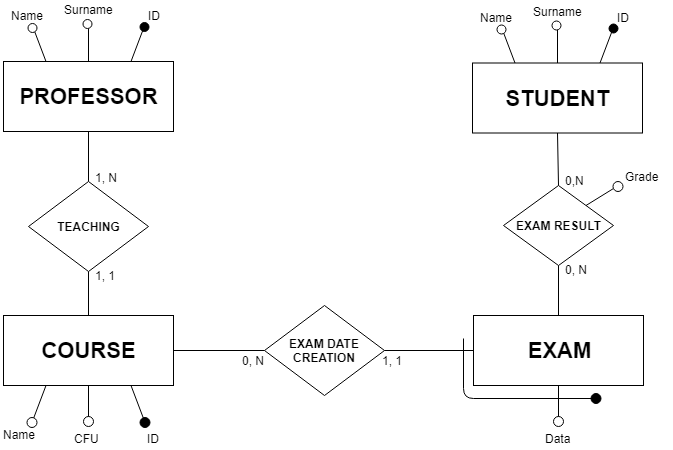
\includegraphics[width=0.9\textwidth]{ER_Diagram.png}
	\caption{Entity - Relationship Diagram}
\end{figure}
\addcontentsline{toc}{section}{Database Implementation}
\section*{Database Implementation}
\begin{figure}[ht]
	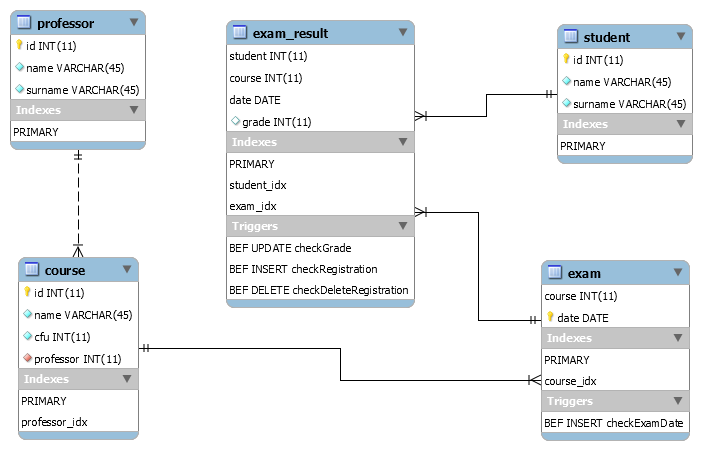
\includegraphics[width=0.85\textwidth]{mysqlSchema.png}
	\caption{MySQL Schema}
\end{figure}

\addcontentsline{toc}{section}{Design and Implementation of Java Application (with JPA)}
\section*{Design and Implementation of Java Application (with JPA)}
\begin{figure}[ht]
	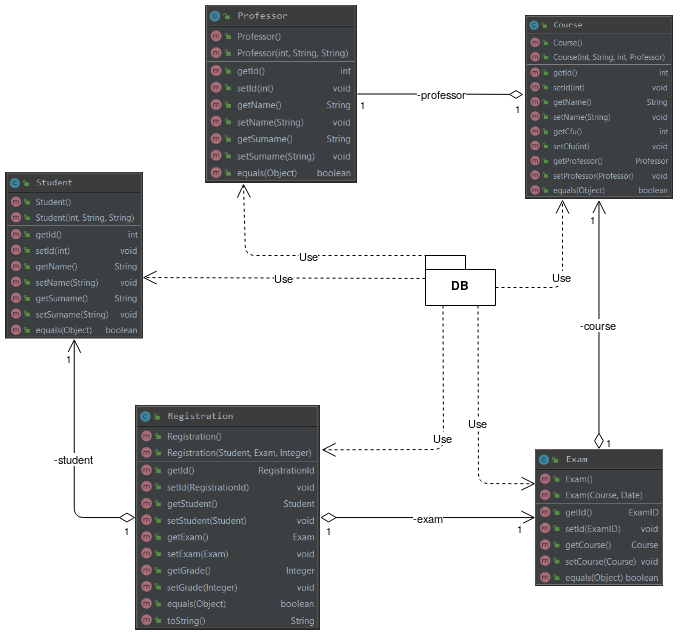
\includegraphics[width=1\textwidth]{Jpa_leveldb_Diagram.png}
	\caption{MySQL Schema}
\end{figure}

\begin{figure}[ht]
	\centering
	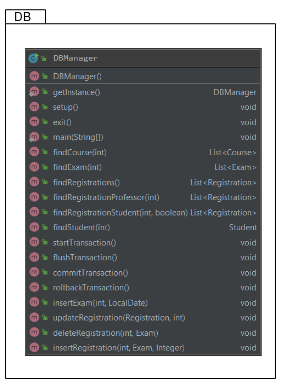
\includegraphics[width=0.6\textwidth]{jpa-DBPackage.png}
	\caption{DBManager class design in task.db Package}
\end{figure}


%\addcontentsline{toc}{chapter}{Implementation}
%\chapter*{Implementation}
Project design and implementation is based on two main packages, \textit{task.db} and \textit{task.gui}, and database class objects implementation.
\addcontentsline{toc}{section}{task.db package}
\section*{task.db package}
This package includes only one class, \textit{DBManager}, which is based on Singleton design pattern. Each method implements a CRUD operation on MySQL database using jpa api methods. A list of all the methods:
\begin{itemize}
	\item public List\(<\)Course\(>\) findCourse(int profID); \newline find all courses given a professor ID
	\item public List\(<\)Exam\(>\) findExam(int studId); \newline find all exams registered by a student indentified by its ID 
	\item public List\(<\)Registration\(>\) findRegistrationProfessor(int profId); \newline find all registrations opened by professor identified by the parameter ID
	\item public List\(<\)Registration\(>\) findRegistrationStudent(int studentId, boolean toDo); \newline find all registrations applied to student identified by student ID. If toDo is true, show only registrations without grade, otherwise return all registration with grade
	\item public void insertExam(int courseID, LocalDate date); \newline add exam for specified courseID at specified date
	\item public void insertRegistration(int studentId, Exam examDetached, @Nullable Integer grade); \newline insert registration for specified student and exam (can be detached from jpa context). grade can be null, in that case it means that a registration is inserted without a grade
	\item public void updateRegistration(Registration reg, int grade); \newline update grade to a registration
	\item public void deleteRegistration(int studentId, Exam exam); \newline delete registration given its key (composite key of studentid + exam)
\end{itemize}

\subsection*{Using of EntityManager and EntityFactoryManager}
\begin{lstlisting}
public class DBManager {
	private static DBManager INSTANCE = new DBManager();
	public static DBManager getInstance() {
		return INSTANCE;
	}

	private EntityManagerFactory factory;

	public DBManager() {
		setup();
	}

	public void setup() {
		factory = Persistence.createEntityManagerFactory("Task0");
	}

	public void exit() {
		factory.close();
	}

	[...]
}
\end{lstlisting}
As we can see, \textit{entityFactory} is only created at setup time (in \textit{setup()}, called by constructor) and closed when the applications get closed (through calling \textit{close()}). In the next code snippets it's showed how \textit{entityManager}, instead, is created from \textit{entityFactory} and closed, respectively, at start and the end of each method that implements CRUD operations on database.
\\

\subsection*{Implementation of findRegistrationStudent(int studentId, boolean toDo)}
This implementation and the following one use JPQL language instead of SQL.
\begin{lstlisting}
public List<Registration> findRegistrationStudent(int studentId, boolean toDo) {
List<Registration> resultList;
	try {
		entityManager = factory.createEntityManager();
		Query query =
			entityManager.createQuery("SELECT r FROM Registration r " +
			"WHERE r.student.id = :studentId AND r.grade IS "
			+ ((toDo) ? "NULL" : "NOT NULL"));
		query.setParameter("studentId", studentId);
		resultList = query.getResultList();
	} catch (Exception ex) {
		throw ex; // Let GUI show the exception
	} finally {
		entityManager.close();
	}

	return resultList;
}
\end{lstlisting}

\subsection*{Implementation of findExam(int studId)}
\begin{lstlisting}
public List<Exam> findExam(int studId) {
	List<Exam> resultList;
	try {
		entityManager = factory.createEntityManager();
		Query query = entityManager.createQuery("SELECT e FROM Exam e "+
			"WHERE (SELECT count(r) FROM Registration r " +
			"WHERE r.student.id = :studId AND r.exam.id = e.id " +
			"OR (r.exam.course = e.course AND r.grade IS NOT NULL) " +
			") = 0");
		query.setParameter("studId", studId);
		resultList = query.getResultList();
	} catch (Exception ex) {
		throw ex;
	} finally {
		entityManager.close();
	}

	return resultList;
}
\end{lstlisting}

\addcontentsline{toc}{section}{task.gui package}
\section*{task.gui package}
Includes classes related to gui implementation, implemented using JavaFX API.

\addcontentsline{toc}{section}{Database object classes Design and Implementation}
\section*{Database object classes Design and Implementation}
Database objects implementation derived from Task0 have been converted to a JPA implementation. Although this phase should have been a simple annotation task, it caused some issues with composite keys implementation. JPA requires that each composite key should be implemented as an @Embeddable class and instanced into the main object class with a @EmbeddedID reference (check tutorial for more details). In addition to this, each composite key member should have a duplicated reference inside the main class, annotated with @MapsID, which realizes the relation of composite key members. Also, JPA specification requires that each entity class must implement a costructor with no parameters. We choosed also to use every annotation on getter and setter methods instead of entity class members, although it does not make any difference, apart from be able to intercept every get and set operation made by JPA, which in any case we don't use. Student and Professor implementation is straighforward.

\subsection*{Student}
\begin{lstlisting}[language=Java]
import javax.persistence.*;

@Entity
@Table(name = "student")
public class Student {
	private int id;
	private String name;
	private String surname;

	public Student() {}

	public Student(int id, String name, String surname) {
		this.id = id;
		this.name = name;
		this.surname = surname;
	}

	@Column(name = "id")
	@Id
	@GeneratedValue(strategy = GenerationType.IDENTITY)
	public int getId() { return id; }

	public void setId(int id) { this.id = id; }
	public String getName() { return name; }
	public void setName(String name) { this.name = name; }
	public String getSurname() { return surname; }
	public void setSurname(String surname) { this.surname = surname; }
}
\end{lstlisting}
Professor implementation is similar to this.


\subsection*{Registration}
\begin{lstlisting}
import javax.persistence.*;
import java.io.Serializable;
import java.sql.Date;

@Entity
@Table(name = "exam_result")
public class Registration {

	@Embeddable
	public static class RegistrationId implements Serializable {
		private int student;
		private Exam.ExamID exam;

		public RegistrationId() {}

		public int getStudent() { return student; }
		public void setStudent(int student) { this.student = student; }
		public Exam.ExamID getExam() { return this.exam; }
		public void setExam(Exam.ExamID exam) { this.exam = exam; }

		@Override
		public boolean equals(Object obj) {
			if(obj == null || obj.getClass() != this.getClass())
				return false;

			RegistrationId regobj = (RegistrationId)obj;
			return student == regobj.getStudent()
				&& exam.equals(regobj.getExam());
		}

		// hashcode should be implemented in case of using
		// @OneToMany relations using HashMaps
		@Override
		public int hashCode() {
			return super.hashCode();
		}
	}



	public Registration () {}
	public Registration (Student student, Exam exam, Integer grade) {
		this.exam = exam;
		this.grade = grade;
		this.student = student;
		this.id = new RegistrationId();
		this.id.setExam(exam.getId());
		this.id.setStudent(student.getId());
	}

	private RegistrationId id;
	@EmbeddedId
	public RegistrationId getId() { return id; }
	public void setId(RegistrationId id) { this.id = id; }

	// ===== Key fields =====
	private Student student;

	@MapsId("student")
	@JoinColumn(name="student", referencedColumnName="id")
	@ManyToOne
	public Student getStudent () { return student; }
	public void setStudent(Student student) { this.student = student; }

	private Exam exam;

	@MapsId("exam")
	// il join tra Registration e Exam va fatto su due campi contemporaneamente:
	// exam_result.course = exam.course AND exam_result.date = exam.date
	@JoinColumns({
			@JoinColumn(name="course", referencedColumnName="course"),
			@JoinColumn(name="date", referencedColumnName="date")
	})
	@ManyToOne
	public Exam getExam() { return this.exam; }
	public void setExam(Exam exam) { this.exam = exam; }

	// ===== Additional fields =====
	private Integer grade;
	@Column(name = "grade")
	public Integer getGrade() { return grade; }
	public void setGrade(Integer grade) { this.grade = grade; }
}
\end{lstlisting}
Exam class implementations is similar to Registration implementation. We showed this to show an example of use of an embedded reference inside an embedded class.



\addcontentsline{toc}{chapter}{Key-Value Feasibility Study}
\chapter*{Key-Value Feasibility Study}
The first version of the application stores all its data in a relational database managed by the MySQL RDBMS.
The main non-functional requirements are availability and consistency ad they are both guaranteed by the relational database since the application handles a limited amount of data.
Availability may be nomore guaranteed if the number of users grows large, i.e. the number of students. The system may responds slower when too many users are active at the same time since in this scenario the relational database has to perform a lot of complex operations to fullfill their demands resulting in not negligible waiting times. \linebreak
Operations that work with exam registrations are the most expensive and time consuming as they require to perform a join on multiple tables of the database. Reducing this kind operations may be a possible solution to improve the system performance: it may be convenient to use a key-value database in parallel with the relational one and spread different operations between them. \linebreak

The relational database still stores all the business data and the key-value database stores only data relative to registrations. The two copies registrations data make the storage system redundant but consistency is always guaranteed by the fact that write operations are committed on both the databases or canceled.
When a write operation occurs both the databases update consistently their data and if one of two can not commit the update the other rollbacks and it is so possible to perform a write operation if and only if both databases are on.
If a read operation regards single-table data it is redirected towards the relational database, if instead it regards registrations it is redirected towards the key-value database. In the latter case it may happen that the key-value database is anavailable, in this case the read operation is redirected towards the relational database. \linebreak 

The key is composed concatenating:
\begin{itemize}
	\item a prefix, ``registration''
	\item id of the course of the exam;
	\item date of the exam;
	\item id of the professor of the course;
	\item id of the student.
	\item value name
\end{itemize}
The full form is \textbf{registration:courseId:date:profId:studentid:valuename}, where \textbf{valuename} can be one of this list:
\begin{itemize}
	\item \textit{studentname}: name of the student;
	\item \textit{studentsurname}: surname of the student;
	\item \textit{professorname}: name of the professor;
	\item \textit{professorsurname}: surname of the professor;
	\item \textit{coursename}: name of the course;
	\item \textit{coursecfu}: number of CFU of the course;
	\item \textit{grade}: grade assigned by the professor. grade null value is mapped to \(-1\) (grade cannot be less than 0)
\end{itemize}
For each registration, this list of key-value is inserted into the database.

\paragraph{Registration LevelDB Entry Example:}
Student Mario Rossi (id = 3) registered to exam with date 2018-08-08 of Programming course (6 cfu, id = 1) with a grade of 29. The course is held by prof. Francesco Bianchi (id = 2). The following key-value pairs (showed in form of \textit{key = value}) will be added to LevelDB database:
\begin{lstlisting}
registration:1:2018-08-08:2:3:coursecfu = 6
registration:1:2018-08-08:2:3:coursename = Programming
registration:1:2018-08-08:2:3:grade = 29
registration:1:2018-08-08:2:3:professorname = Francesco
registration:1:2018-08-08:2:3:professorsurname = Bianchi
registration:1:2018-08-08:2:3:studentname = Mario
registration:1:2018-08-08:2:3:studentsurname = Rossi
\end{lstlisting}

A key-value database is used to take advantage of its semplicity and velocity to speedup read operations on regitrations data.

\addcontentsline{toc}{section}{Class Design and Implementation}
\section*{Class Design and Implementation}
\subsection*{LevelDBManager class}
As we previously mentioned, LevelDB should support MySQL DB on registration queries. The first step is to design and implement a manager class, similar to DBManager, called \textit{LevelDBManager}, which must implement a subset of DBManager methods, in particular all methods related to registration handling:
\begin{lstlisting}
public void addRegistration(Registration registration);
public void updateRegistration(Registration reg, @Nullable Integer grade);
public void insertRegistration(Student student, Exam exam, @Nullable Integer grade);
public List<Registration> findRegistrationProfessor(int professorId);
public List<Registration> findRegistrationStudent(int studentId, boolean toDo);
\end{lstlisting}
Method implementations is not showed here due to code length.

\addcontentsline{toc}{subsection}{Strict consistency implementation with Transactions}
\subsection*{Strict consistency implementation with Transactions}
To manage strict consistency, it is required that at least one of the two Manager classes has to implement transactions on registration methods. The common case is the following: a write operation is executed and SQL and LevelDB databases should both execute the operation. If SQL query execution is successful but it is not he same for LevelDB, then the SQL query should be reverted. The same is if LevelDB is successful but SQL is not. To speedup write operations, we can think to parallelize both writes and commit only when both are successful. Unluckily this is not a possible choice, because LevelDB does not implement any form of transaction. This means that the only way to mantain strict consistency on all the CRUD operations on registrations is to first perform the query on the SQL database, without committing, then to execute the query on LevelDB. If both the operations are successful, then commit on SQL database can be performed, otherwise it rollbacks. In pseudo-code:
\begin{lstlisting}
	function writeop() {
		try {
			DBManager.begin();		// start transaction
			DBManager.writeop(); 	// perform on SQL database first
			LevelDB.writeop();		// performed always after SQL query
			DBManager.commit();		// if we are here both query are correct
		} catch {
			DBManager.rollback(); // rollback on all exceptions
		}
	}
\end{lstlisting}

\addcontentsline{toc}{subsubsection}{Transactions on DBManager (SQL)}
\subsubsection{Transactions implementation in DBManager (SQL)}
All registration write methods (update, insert and delete) must implement transactions. As we are using JPA with resource-local entityManager(s), the only choice is to use EntityTransaction class methods. For each operation we must:
\begin{enumerate}
	\item Create a new entityManager from entityFactory
	\item Get a EntityTransaction instance from entityManager
	\item Start a transaction (using EntityTransaction)
	\item Perform all the operations
	\item Commit or Rollback transaction (using EntityTransaction)
	\item Close the entityManager
\end{enumerate}
Also, we want to let external classes to be able to manage transactions, so this means that we must add some public methods for begin, commit and rollback operation on current transaction and not use this methods in DBManager methods themself. In this case, entityManager persists over multiple method calls, so it must be defined as a member of DBManager. However we don't want to mix previously defined methods for exam, student, professor and so on, with those new implementation of registration methods, due to the fact that in the previous ones, entityManager gets created and closed in each single method. So, to differentiate this two subsets, we implemented an additional Transactions class, which is an inner class of DBManager. This class has a member entityManager and can access entityManagerFactory of the outer class.


\begin{figure} [h!]
	\centering
	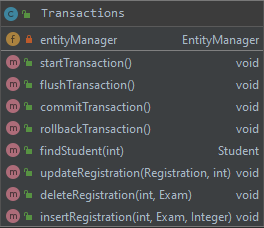
\includegraphics[width=0.5\textwidth]{TransactionsClassDia.png}
	\caption{Transactions Class Diagram}
	\label{fig:transactions-dia}
\end{figure}

Follows our implementation of Transaction Class with just one database method for registrations:
\begin{lstlisting}
public class DBManager {
	private EntityManagerFactory factory;

	public class Transactions {
		[...]
		private EntityManager entityManager;
		public void startTransaction() {
			entityManager = factory.createEntityManager();
			entityManager.getTransaction().begin();
		}

		public void commitTransaction() {
			entityManager.getTransaction().commit();
			entityManager.close();
		}

		public void rollbackTransaction() {
			entityManager.getTransaction().rollback();
			entityManager.close();
		}

		public void flushTransaction() {
			entityManager.flush();
		}

		public void deleteRegistration(int studentId, Exam exam) {
			try {
				Query query = entityManager
					.createQuery("DELETE FROM Registration r WHERE "+
					" r.exam = :exam AND r.student.id = :studId");
				query.setParameter("exam", exam);
				query.setParameter("studId", studentId);
				query.executeUpdate();
			} catch (Exception ex) {
				ex.printStackTrace();
				System.out.println("Exception on delete registration!");
				throw ex;
			}
		}

		[.. Other Methods to use WITH transactions ..]
	}

	[.. Methods to use WITHOUT transactions ..]
}
\end{lstlisting}
As we can see, entityManager lifecycle management is now a responsibility of the external class which performs any call on DBManager methods. The entityManager is created for each startTransaction() call and closed on rollback and commit.
At this point, any external class can use and define transactions for DBManager.Transactions methods.

\addcontentsline{toc}{subsubsection}{EntityTransactions and Trigger Errors}
\subsubsection{JPA and Trigger Error management}
An issue occurred during testing of triggers on our JPA implementation: using the previous pseudo-code, as it is, it can cause to break strict consistency due to the fact that the effective query execution happens on commit() instead of the writeop() itself, leading to unwanted finalized writes on LevelDB database. To solve this, we must add a flush() call after calling DBManager write methods, forcing to execute all the queued queries. The new pseudo-code is this:
\begin{lstlisting}
	function writeop() {
		try {
			DBManager.begin();		// start transaction
			DBManager.writeop(); 	// perform on SQL database first
			DBManager.flush();		// <== FLUSH TO GET ANY TRIGGER ERROR HERE
			LevelDB.writeop();		// performed always after SQL query
			DBManager.commit();		// if we are here both query are correct
		} catch {
			DBManager.rollback(); // rollback on all exceptions
		}
	}
\end{lstlisting}


\addcontentsline{toc}{subsubsection}{Orchestration with CompositeDBManager class}
\subsubsection*{Orchestration with CompositeDBManager class}
To better organize all the code related to the orchestration of LevelDBManager and DBManager class, we defined a new class, called CompositeDBManager, which implements the same public interface of DBManager and handles all the cases we just defined. This means that this class will be the connecting code entity between the GUI and the database layer, basically taking the role of DBManager class. All read operations, in addition to all write operations on entities different from \textit{registration} are simply passed to DBManager without any pre/post processing. For all the remaining operations, we use the last approach described with pseudo code. Let's show an example:
\begin{lstlisting}
public class CompositeDBManager {
	[...]
	public void updateRegistration(Registration reg, int grade)
			throws SQLException, LevelDBUnavailableException,
			InconsistentDatabaseException {
		try {
			DBManager.transactions().startTransaction();
			lastExecutor = QueryExecutor.Both;
			DBManager.transactions().updateRegistration(reg, grade);
			DBManager.transactions().flushTransaction();
			levelDBManager.updateRegistration(reg, grade);
			DBManager.transactions().commitTransaction();
		} catch (Exception e) {
			DBManager.transactions().rollbackTransaction();
			throw e;
		} finally {
			checkConsistency();
		}
	}
}
\end{lstlisting}
We will see \textit{LevelDBUnavailableException}, \textit{InconsistentDatabaseException} and checkConsistency() in Testing section. \textit{lastExecutor} is a member variable used to display on GUI which is the executor for the last query (MySQL, LevelDB or both), so it's just used for debugging purposes.

\newpage
\addcontentsline{toc}{subsection}{UML Class Diagram for task.db package}
\subsection*{UML Class Diagram for task.db package}
\begin{figure} [!ht]
	\centering
	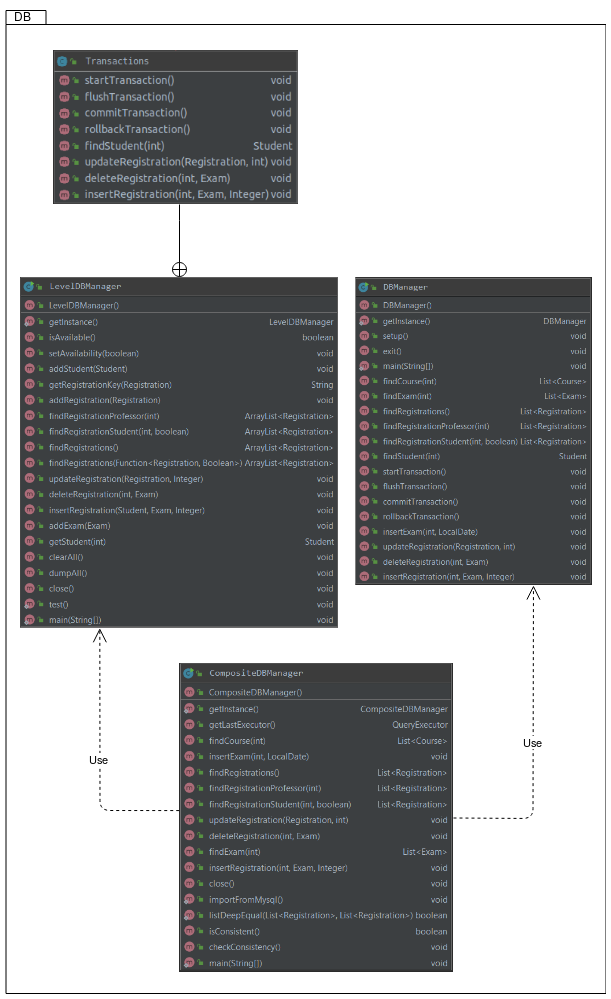
\includegraphics[width=0.8\textwidth]{jpaLevelDB-DBPackage.png}
	\caption{UML Class Diagram for task.db package}
	\label{fig:leveldb-classdia}
\end{figure}


\addcontentsline{toc}{section}{Testing}
\section*{Testing}
Testing code is important here to check if \textbf{strict consistency is correctly achieved} after executing any type of database operation.

\addcontentsline{toc}{subsection}{Testing methods}
\subsection*{Testing methods}
DBManager, LevelDBManager and CompositeDBManager all implements a main() method which perform a \textbf{suite of tests}. In particular, CompositeDBManager tries to load all the registrations from MySQL database into LevelDB database, then tries to get them from LevelDB and check if the initial list and the obtained list are equals. This led to some implementation issues, due to the fact that Java does not provide a method to \textbf{compare lists deeply}. Also, not all of database object classes overrode equals() method, and this required to implement them all.

\addcontentsline{toc}{subsection}{Strict consistency checks}
\subsection*{Strict consistency checks}
After each CompositeManagerDB call on registration write methods, we can perform the same consistency check we just defined: take registration list from database, take registration list from LevelDB and the compare them deeply. We expect that every write operation on registrations passes this check.
\begin{lstlisting}
boolean isConsistent() throws SQLException, LevelDBUnavailableException {
	return listDeepEqual(DBManager.getInstance().findRegistrations(),
							LevelDBManager.getInstance().findRegistrations());
}

void checkConsistency() throws SQLException, InconsistentDatabaseException {
	try {
		if(!isConsistent())
			throw new InconsistentDatabaseException(
				"LevelDB/MySQL database is inconsistent! This should not happen");
	} catch (LevelDBUnavailableException e) {
		System.out.println("Cannot check consistency: LevelDB is unavailable");
	}
}
\end{lstlisting}
An example of checkConsistency() call can be seen in previous code chunks.\\
NOTE: this check cannot be used in deployment because is too performance heavy. We did not remove all checking calls just for debugging purporses and \textbf{they can be removed without affecting application functionalies}.

\addcontentsline{toc}{subsection}{LevelDB Exception simulation}
\subsection*{LevelDB Exception simulation}
LevelDB operations can lead to \textbf{exceptions}, but they are not so simple to trigger when we want to test them. To solve the problem, we decided to ``simulate'' exceptions, triggering them at command.\\
We defined a simple \textbf{LevelDBUnavailableException} class, which triggers the exception any time a method from leveldb sees that the member variable \textbf{LevelDBManager.isAvailable }is set to \textbf{true}.\\
This member variable can be changed directly from the GUI.


\addcontentsline{toc}{chapter}{User's Manual}
\chapter*{User's Manual}
The application starts and shows a minimal user interface, fig. \ref{fig:UIStart},
\begin{figure}[h!]
	\centering
	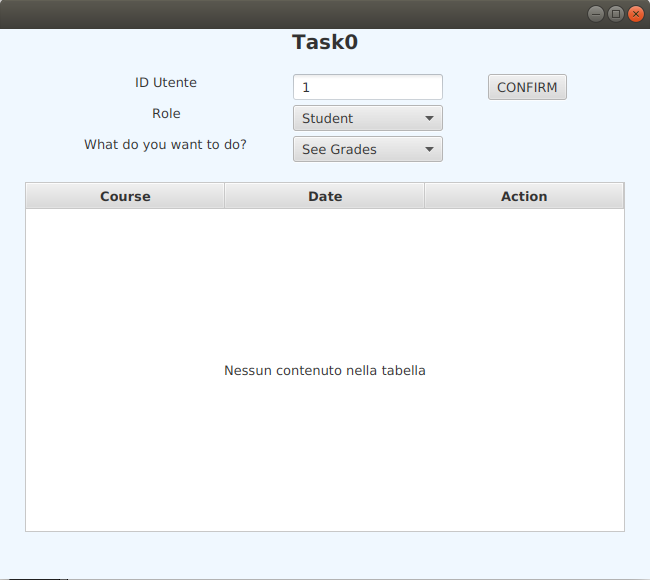
\includegraphics[width=0.7\textwidth]{UIStart.png}
	\caption{User Interface when the application starts}
	\label{fig:UIStart}
\end{figure}
composed of:
\begin{itemize}
	\item \textit{UserID} field, where the user specifies his id number;
	\item \textit{Role} choise box, whith the option:
	\begin{enumerate}
		\item Professor, in case the user is a Professor;
		\item Student, in case the user is a Student.
	\end{enumerate} 
	\item \textit{What do you want to do?} choise box, where the user specifies the action he wants to perform. The options change according to the role chosen.
	Professor can select among:
	\begin{enumerate}
		\item \textit{Add Exam} if he wants to add an exam;
		\item \textit{Add Grade} if he wants to add a grade.
	\end{enumerate}
	A Student can select among:
	\begin{enumerate}
		\item \textit{Register to Exam} if he wants to register to an exam;
		\item \textit{Deregister to Exam} if he wants to deregister to an exam;
		\item \textit{See Grades} if he wants to see the grades he got.
	\end{enumerate}
	\item \textit{Confirm} button;
	\item A table showing the results of the selected operation. The layout of the table can change according depending on the selected operation.
\end{itemize}
\section*{Professor}
A Professor:
\begin{enumerate}
	\item Inserts his ID number into the \textit{UserID} field;
	\item Selects \textsl{Professor} in the \textit{Role} choise box;
	\item Selects the action he wants to perform;
	\item Pushes the \textit{Confirm} button.
\end{enumerate}
\subsubsection*{Add Exam}
If the Professor select the \textit{Add Exam} option, the table, fig. \ref{fig:AddExam}, is populated with a list of all the courses he is currently holding. Each element of the list is composed of:
\begin{figure} [h!]
	\centering
	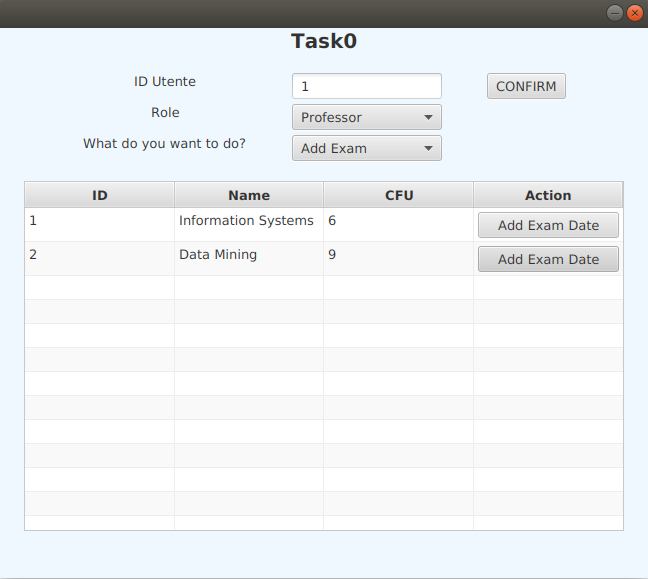
\includegraphics[width=0.7\textwidth]{AddExam.png}
	\caption{Example of Add Exam}
	\label{fig:AddExam}
\end{figure}
\begin{itemize}
	\item \textit{ID}, the id of the course;
	\item \textit{Name}, the name of the course;
	\item \textit{CFU}, the number of credits assigned to the course;
	\item \textit{Add Exam Date}, button the professor has to push in order to add an exam corresponding to the course. 
\end{itemize}

If the Professor pushes one of the \textit{Add Exam Date} buttons a confirm dialog is presented and it asks for the date of the exam to insert, fig. \ref{fig:AddExamDialog.png}.
\begin{figure} [h!]
	\centering
	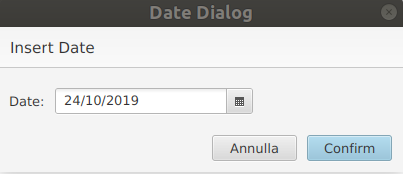
\includegraphics[width=0.5\textwidth]{AddExamDialog.png}
	\caption{Example of Add Exam dialog}
	\label{fig:AddExamDialog}
\end{figure} 
If the Professor wants to confirm he:
\begin{enumerate}
	\item Selects the date using the datepicker;
	\item Pushes the \textit{Confirm} button in the dialog.
\end{enumerate}
To go back and undo the operation the Professor just pushes the \textit{Delete} button.
\subsubsection*{Add Grade}
If the Professor select the \textit{Add Grade} option, the table, fig. \ref{fig:AddGrade}, is populated with a list of all the registrations to the courses he is currently holding. Each element of the list is composed of:
\begin{figure} [h!]
	\centering
	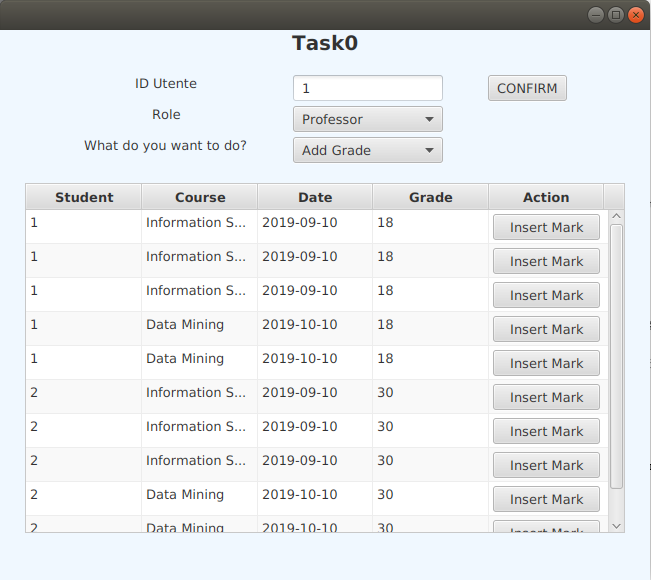
\includegraphics[width=0.7\textwidth]{AddGrade.png}
	\caption{Example of Add Grade}
	\label{fig:AddGrade}
\end{figure}
\begin{itemize}
	\item \textit{Student}, the id of the student enrolled to the exam;
	\item \textit{Course}, the name of the course;
	\item \textit{Date}, the date of the exam;
	\item \textit{Insert Mark} button that the professor has to push in order to insert a grade to the corresponding registration. 
\end{itemize}
If the Professor pushes one of the \textit{Insert mark} buttons a confirm dialog is presented and it asks for the grade of the exam to insert, fig. \ref{fig:AddGradeDialog}.
\begin{figure} [h!]
	\centering
	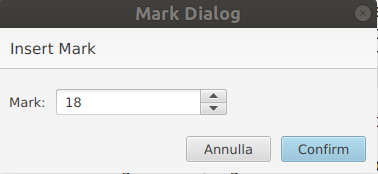
\includegraphics[width=0.5\textwidth]{AddGradeDialog.png}
	\caption{Example of Add Grade dialog}
	\label{fig:AddGradeDialog}
\end{figure}
If the Professor wants to confirm he:
\begin{enumerate}
	\item Inserts the grade in the corresponding field;
	\item Pushes the \textit{Confirm} button in the dialog.
\end{enumerate}
To go back and undo the operation the Professor just pushes the \textit{Delete} button.

\section*{Student}
A Student:
\begin{enumerate}
	\item Inserts his ID number in the \textit{UserID} field;
	\item Selects \textsl{Student} in the \textit{Role} choise box;
	\item Selects the action he wants to perform;
	\item Pushes the \textit{Confirm} button.
\end{enumerate}
\subsubsection*{Register to Exam}
If the Student select the \textit{Register to Exam} option, the table, fig. \ref{fig:RegisterToExam}, is populated with a list of all the available exams. Each element of the list is composed of:
\begin{figure} [h!]
	\centering
	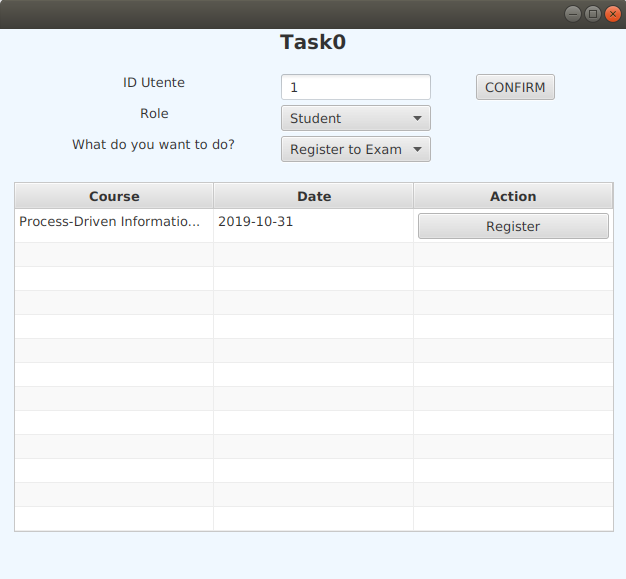
\includegraphics[width=0.7\textwidth]{RegisterToExam.png}
	\caption{Example of Register to Exam}
	\label{fig:RegisterToExam}
\end{figure}
\begin{itemize}
	\item \textit{Course}, the name of the course;
	\item \textit{Date}, the date of the exam;
	\item \textit{Register}, button the student has to push in order to register to the selected exam. 
\end{itemize}
If the Student pushes one of the \textit{Register to Exam} the table is updated so that it shows all the exams to which the Student is not enrolled.

\subsubsection*{Deregister to Exam}
If the Student select the \textit{Deregister} option, the table, fig. \ref{fig:DeregisterToExam}, is populated with a list of all the registrations corresponding to the Student. Each element of the list is composed of:
\begin{figure} [h!]
	\centering
	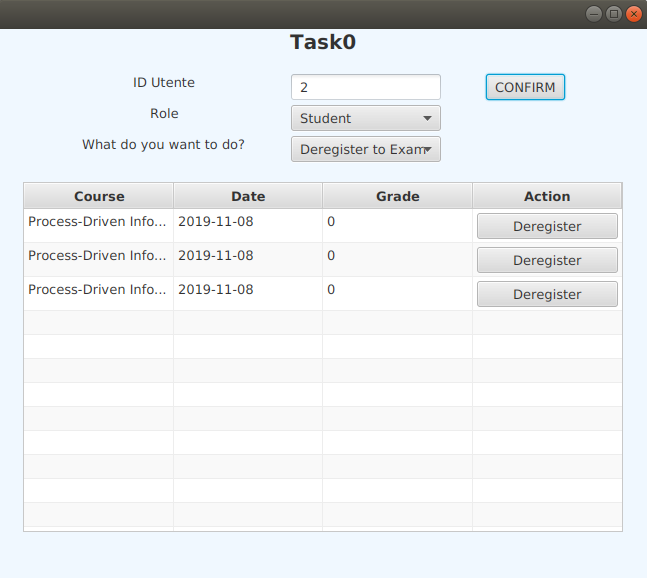
\includegraphics[width=0.7\textwidth]{DeregisterToExam.png}
	\caption{Example of Deregister to Exam}
	\label{fig:DeregisterToExam}
\end{figure}
\begin{itemize}
	\item \textit{Course}, the name of the course of the exam the Student is enrolled to;
	\item \textit{Date}, the date of the exam;
	\item \textit{Deregister} button that the Stuedent has to push in order to do the deregistration. 
\end{itemize}
If the Professor pushes one of the \textit{Deregister} the table is updated so that it shows all the exams to which the Student is not enrolled.

\subsubsection*{See Grades}
If the Student select the \textit{See Grades} option, the table, fig. \ref{fig:SeeGrades}, is populated with a list of all the exams the student has done. Each element of the list is composed of:
\begin{figure} [h!]
	\centering
	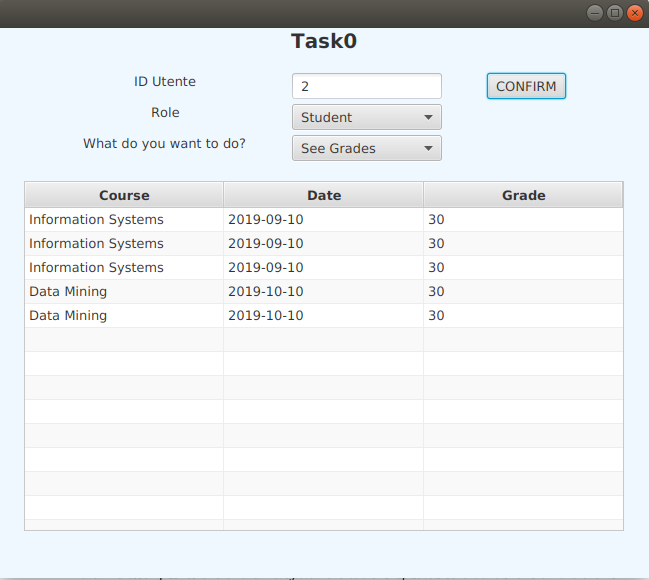
\includegraphics[width=0.7\textwidth]{SeeGrades.png}
	\caption{Example of See Grades}
	\label{fig:SeeGrades}
\end{figure}
\begin{itemize}
	\item \textit{Course}, the name of the course;
	\item \textit{Date}, the date when the student passed the exam;
	\item \textit{Grade}, the grade the Student got. 
\end{itemize}

\newpage
\section*{LevelDB Handling Example}
The introduction of the LevelDB Key-Value Database required the \textbf{addition of an element} to the GUI. This addition consist of a \textbf{button} at the bottom of the application window, from which the user is able to \textbf{enable or disable} the functionalities provided by LevelDB.\\ 
In particular, since the application is built on a\textbf{ Strict Consistency} requirement, this button's purpose is to \textbf{simulate a malfunctioning} in LevelDB, which makes impossible to write on it. For this reason, all the operations that require to write something cannot be performed, or the\textbf{ Consistency would be lost.}
\begin{figure} [h!]
	\centering
	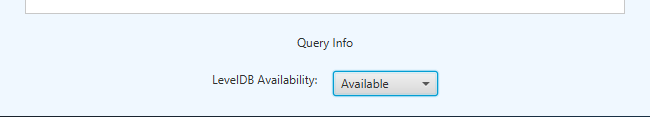
\includegraphics[width=0.7\textwidth]{LevelDBAvailable.png}
	\caption{Enabling LevelDB support }
	\label{fig:LevelDBAvailable}
\end{figure}
\begin{figure} [h!]
	\centering
	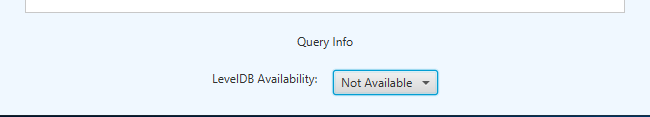
\includegraphics[width=0.7\textwidth]{LevelDBNotAvailable.png}
	\caption{Disabling LevelDB support}
	\label{fig:LevelDBNotAvailable}
\end{figure}

In order to show how this procedure works, we will go through one of the previous use cases, but this time disabling the LevelDB support. We will choose a use case that involves writing on Registrations, in particular the \textbf{Student - Register to Exam}
\subsection*{Student - Register to Exam}
If the Student selects the \textit{Register to Exam} option, the table is populated with a list of all exams the student can register to, as shown in fig \ref{fig:RegisterToExamNotAvailable}.\\
After pressing the \textit{Confirm} button, we will disable the LevelDB support, selecting the option \textit{Not Available} from the dropdown menu at the bottom of the window, as shown in fig. \ref{fig:LevelDBNotAvailable}.
\begin{figure} [h!]
	\centering
	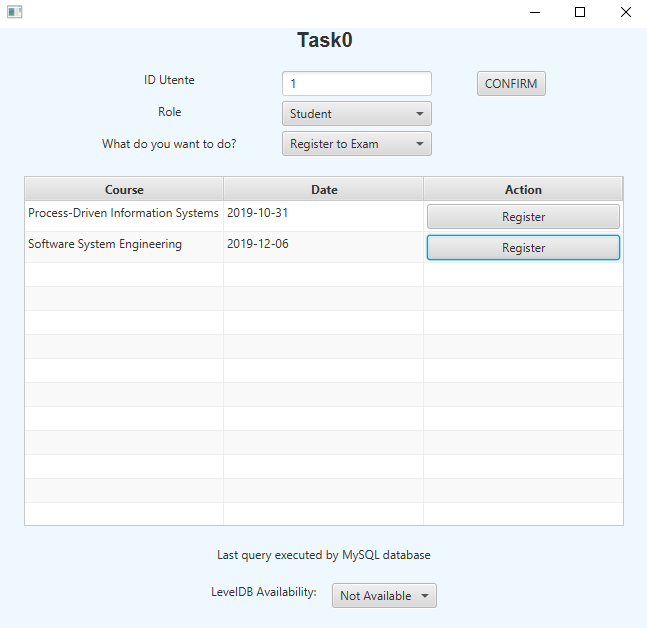
\includegraphics[width=0.8\textwidth]{RegisterToExamNotAvailable.png}
	\caption{Example of Register to Exam without LevelDB support}
	\label{fig:RegisterToExamNotAvailable}
\end{figure}
If then we try to press the \textit{Register} button on the second row of the table, the registration will abort, showing a dialog box with an error message, as in fig. \ref{fig:LevelDBErrorDialog}
\begin{figure} [h!]
	\centering
	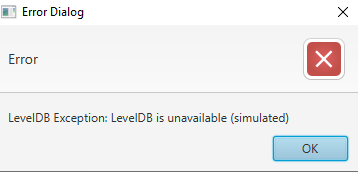
\includegraphics[width=0.6\textwidth]{LevelDBErrorDialog.png}
	\caption{Example of Register to Exam without LevelDB support}
	\label{fig:LevelDBErrorDialog}
\end{figure}




\end{document}
